
\documentclass[
10pt,
a4paper, 
oneside, 
headinclude,footinclude, 
]{scrartcl}

%%%%%%%%%%%%%%%%%%%%%%%%%%%%%%%%%%%%%%%%%
% Arsclassica Article
% Structure Specification File
%
% This file has been downloaded from:
% http://www.LaTeXTemplates.com
%
% Original author:
% Lorenzo Pantieri (http://www.lorenzopantieri.net) with extensive modifications by:
% Vel (vel@latextemplates.com)
%
% License:
% CC BY-NC-SA 3.0 (http://creativecommons.org/licenses/by-nc-sa/3.0/)
%
%%%%%%%%%%%%%%%%%%%%%%%%%%%%%%%%%%%%%%%%%

%----------------------------------------------------------------------------------------
%	REQUIRED PACKAGES
%----------------------------------------------------------------------------------------

\usepackage[
nochapters, % Turn off chapters since this is an article        
beramono, % Use the Bera Mono font for monospaced text (\texttt)
eulermath,% Use the Euler font for mathematics
pdfspacing, % Makes use of pdftex’ letter spacing capabilities via the microtype package
dottedtoc % Dotted lines leading to the page numbers in the table of contents
]{classicthesis} % The layout is based on the Classic Thesis style

\usepackage{arsclassica} % Modifies the Classic Thesis package

\usepackage[T1]{fontenc} % Use 8-bit encoding that has 256 glyphs

\usepackage[utf8]{inputenc} % Required for including letters with accents

\usepackage{graphicx} % Required for including images
\graphicspath{{Figures/}} % Set the default folder for images

\usepackage{enumitem} % Required for manipulating the whitespace between and within lists

\usepackage{lipsum} % Used for inserting dummy 'Lorem ipsum' text into the template

\usepackage{subfig} % Required for creating figures with multiple parts (subfigures)

\usepackage{amsmath,amssymb,amsthm} % For including math equations, theorems, symbols, etc

\usepackage{varioref} % More descriptive referencing
\usepackage{siunitx}
\usepackage{makeidx}
\makeindex
\usepackage{glossaries}
\makeglossaries
%----------------------------------------------------------------------------------------
%	THEOREM STYLES
%---------------------------------------------------------------------------------------

\theoremstyle{definition} % Define theorem styles here based on the definition style (used for definitions and examples)
\newtheorem{definition}{Definition}

\theoremstyle{plain} % Define theorem styles here based on the plain style (used for theorems, lemmas, propositions)
\newtheorem{theorem}{Theorem}

\theoremstyle{remark} % Define theorem styles here based on the remark style (used for remarks and notes)

%----------------------------------------------------------------------------------------
%	HYPERLINKS
%---------------------------------------------------------------------------------------

\hypersetup{
%draft, % Uncomment to remove all links (useful for printing in black and white)
colorlinks=true, breaklinks=true, bookmarks=true,bookmarksnumbered,
urlcolor=webbrown, linkcolor=RoyalBlue, citecolor=webgreen, % Link colors
pdftitle={}, % PDF title
pdfauthor={\textcopyright}, % PDF Author
pdfsubject={}, % PDF Subject
pdfkeywords={}, % PDF Keywords
pdfcreator={pdfLaTeX}, % PDF Creator
pdfproducer={LaTeX with hyperref and ClassicThesis} % PDF producer
}


 
\newglossaryentry{SA}{
name={SOTA},
description={State of the art. Défini les standards les plus exigents de l’industrie et notamment pour la recherche, dans le domaine de la vision par ordinateur}
}

\newglossaryentry{DLV3}{
name={DeepLabV3},
description={Algorithme de deep learning utilisant le principe d’encodeur et décodeur avec des convolutions séparables Atrous pour la segmentation sémantique d’image}
}

\newglossaryentry{FEATS}{
name={features},
description={Singularités dans l’image, capturées à travers des filtres et à des échelles multiples, puis pouvant être mises en correspondance entre les niveaux pour obtenir des prédictions de classes d’appartenance pour chaque pixel de l’image. Chaque singularités capturées pouvant servir d’entrée dans une autre sous-partie du réseau de neurones à des fins de délimitation de frontière d’objets plus ou moins diffus de l’image comme par exemple le ciel ou un véhicule}
}

\newglossaryentry{FCN}{
name={FCN},
description={Ce sont des réseaux convolutifs ou "convnets", qui sont complètement connectés, i.e. chaque neurone de sortie est connecté aux neurones d’entrée. Ils permettent non seulement la classification de l’image entière, mais en en ayant permis des progrès sur les tâches locales, pourvoyant des outputs structurés}
}


\newglossaryentry{MIOU}{
name={mIoU},
description={La moyenne d’une « Intersection over Union » (IoU), aussi connue sous le nom de l’index Jaccard, est la métrique d’évaluation la plus populaire pour la tâche de segmentation, de la détection d’objet ainsi que du suivi}
}

\newglossaryentry{CFM}{
name={CFM},
description={C’est une méthode (et même un outil), qui relie des extractions de features issues de la convolution puis ensuite, extrait des segments depuis des cartes de features plutôt qu’à partir d’une image brute. Ces segments donnés par R-CNN, sont projetés sur la dernière couche. Les segments projetés jouent un rôle de fonction binaire : les features masquées sont transmises à la couche complètement connectée (fully-connected) pour la reconnaissance}
}


\hyphenation{Fortran hy-phen-ation} 
\title{\normalfont\spacedallcaps{Segmentation sémantique d’image}}


\author{\spacedlowsmallcaps{Romain BOYRIE}}
\date{$17$ Février $2022$} 

\begin{document}


\renewcommand{\sectionmark}[1]{\markright{\spacedlowsmallcaps{#1}}} 
\lehead{\mbox{\llap{\small\thepage\kern1em\color{halfgray} \vline}\color{halfgray}\hspace{0.5em}\rightmark\hfil}} 

\pagestyle{scrheadings} 


\maketitle 

\setcounter{tocdepth}{2} 

\tableofcontents 

\listoffigures

\listoftables 

\newpage
\section*{Abstract} 

Ce document détaille l’étendue des prolégomènes du domaine de la segmentation sémantique d’image sur une architecture basée en réseau neuronal profond. À cet effet, nous avons parcouru, pour les résumer, des papiers scientifiques, en profitant de leur disponibilité, sur le site Arxiv. À ceux-là nous avons ajouté une présentation de nos modèles en exposant notre démarche et nos résultats. Dans un premier temps, nous expliquons pourquoi le champ de la segmentation d’image est lié aux réseaux convolutifs en passant en revue l’état de l’art (\gls{SA}) en le contextualisant avec la recherche, de manière synthétique et pour notre cas particulier, i.e. avec des réseaux comme Xception ou ResNet 50. Dans un second temps, nous parlons de la préparation de nos données et de quelques-unes des solutions que nous avons élaborées en \index{Deep Learning}apprentissage profond. Enfin, dans un troisième temps, nous présentons les résultats de l’architecture qui se démarque dans nos expériences, \index{DeepLabV3}\gls{DLV3}, laquelle a réalisé $62.1\%$ \index{mIoU}\gls{MIOU} (mean of intersection over union) et $71\%$ de coefficient \index{S{\o}rensen-Dice}\gls{Dice} sur la base Cityscapes, avec une augmentation de données.



\section{Segmentation Sémantique}
\paragraph{}À partir des \index{R-CNN}\gls{R-CNN}, La segmentation sémantique classifie chaque pixel en un nombre fixe de catégories mais sans différentiation du nombre d’instance, ce paramètre n’étant pas pris en compte dans la tâche de segmentation. Cette dernière traite de l’identification ou de la classification d’objets similaires en une seule et même classe au niveau du pixel, bien qu’il puisse se trouver plusieurs classes d’objets dans une image.\\
Les Masques R-CNN, qui sont la traduction en calque d’une segmentation d’image, ont été construits en utilisant le \index{Faster R-CNN}\gls{FasterR-CNN}. Toutefois, alors que le Faster R-CNN a 2 sorties pour les objets (un label de classe et un cadre délimitant l’objet), les Masques R-CNN sont l’addition d’une troisième branche dont la sortie est le masque d’objet(s).
\\
Ce masque de sortie est distinct de la classe des cadres délimiteurs d’objets. Ils requièrent l’extraction d’une délimitation en plus, de l’objet dans l’espace, par un calque. Les Masques \index{R-CNN}R-CNN sont une extension des \index{Faster R-CNN}Faster R-CNN et fonctionnent en ajoutant une branche de prédiction d’un calque d’objet (Région d’Intérêt) en parallèle d’une branche existante, car cet ajout délimite les limites encadrant l’objet reconnu dans l’image.


\section{Les Réseaux Convolutifs}

\paragraph{}LeNet est le premier réseau convolutif, lequel fut créé par Bell Labs.
La fin des années 1980 et le début des années 1990 sont le moment du développement des réseaux de neurones multicouches.\\
Cependant, ce n’est qu’en 2012 que cette technologie montre concrètement des résultats impressionnants. C’est cette année-là que l’équipe de Geoffrey Hinton de l’Université de Toronto devient le SOTA avec 16\% d’erreurs sur la base ImageNet (5 catégories, 1,3 million d’images). Le réseau convolutif est, à ce moment-ci, programmé sur une carte GPU.
\begin{figure}[htb]
\centering 
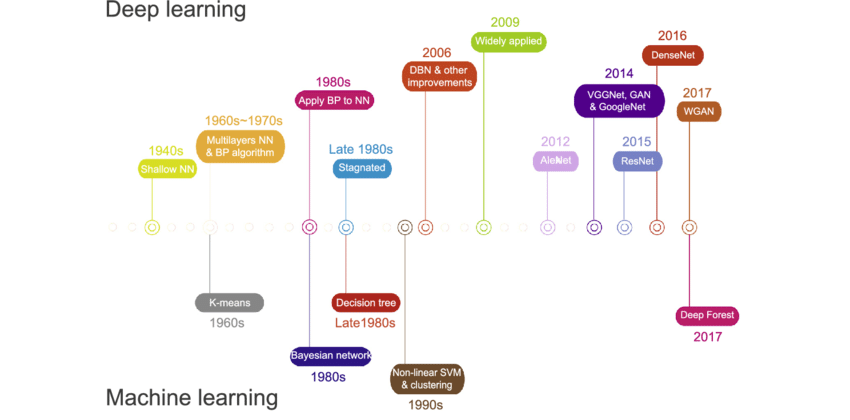
\includegraphics[width=1\columnwidth]{Timeline-of-the-development-of-deep-learning-and-commonly-used-machine-learning} 
\caption[Chronologie des Algorithmes d’Apprentissages]{Chronologie des algorithmes d’apprentissages.} 
\label{fig:gallery} 
\end{figure}
\paragraph{}Le réseau convolutif a des similarités avec la vision du cortex des mammifères. Ces derniers détectent des motifs quelque-soient leurs positions dans l’image (invariance par translation : Pooling), et affectent des millions de neurones à cette tâche et pour toutes les orientations de motifs, lesquels sont les contours des objets de l’image.
Grâce au chercheur japonais Kunihiko Fukushima, qui a travaillé en allant plus loin que le modèle \index{Hubel}\index{Wiesel}d’Hubel et Wiesel$^{1}$\let\thefootnote\relax\footnotetext{1. \textit{i.e. Ils prouvèrent que les aires du cortex visuel primaire jouent le rôle d’un extracteur de caractéristique.}}, un pas est franchi : la progression dans le réseau passe de couche en couche et entraîne la dernière couche mais la rétropropagation n’existe pas encore\cite{LeCun_1998_gblatdr}. \\Ces travaux, dont on ne comprend pas bien la cause, sont peu acceptés par la communauté scientifique. Pourtant, ils seront une source d’inspiration pour la création des extracteurs de caractéristiques \index{SIFT}\gls{SIFT} ou \index{HOG}\gls{HOG}. Notons que ces algorithmes ne sont pas des réseaux de neurones mais une série de calculs complexes.
\paragraph{}Les réseaux convolutifs mélangent dans leur architecture, des cellules simples et complexes (semblables au cortex visuel), mais l’entraînement du système est munit d’une rétropropagation de gradient, donc chaque couche est entraînée pour la reconnaissance de contours.
\paragraph{}Chaque couche de convolution utilise une fenêtre se déplaçant sur l’image, dans laquelle chaque neurone va tenter de détecter un motif qui lui est propre, partout dans l’image. Cela donne une feature map (carte de caractéristique). Chaque feature map de sortie, est la somme de convolutions effectuées sur les "features maps" d’entrée avec des noyaux différents.

Ci-joint le programme d’une couche complète de convolution \cite{LeCun_2019_qlma} :

\inputminted[
frame=lines,
framesep=2mm,
baselinestretch=1,
fontsize=\footnotesize,
linenos=true,
firstnumber=last
]{python}{code/conv.py}

L’opération de convolution passe dans un \index{ReLu}\gls{ReLU} pour mettre en évidence ce qui est détecté, et c’est naturellement que le ReLU est suivi par un Pooling, puisque ce dernier permet de produire des représentations d’invariants, lesquels améliorent la sortie des neurones (malgré les petites variations à l’intérieur d’une fenêtre).

L’architecture typique d’un réseau convolutif est : \\
Conv -> ReLU -> Pool -> Conv -> ReLU -> Pool -> Conv -> ReLU -> Conv

\section{Les Réseaux et ImageNet}

\paragraph{}Il y a plusieurs réseaux existants, lesquels ont représentés le SOTA\ref{fig:Famous_neural_networks}. Pour notre segmentation d’image, nous avons codé implicitement un apprentissage standard sur une structure U-Net avec Xception\ref{fig:Unet_Xception}, mais nous avons poussé plus loin, c’est-à-dire que nous avons utilisé la méthode de \index{Transfer Learning}\gls{Transferlearning} avec le réseau \index{ResNet-50} ResNet-50 sur une structure de \index{DeepLabV3}DeepLabV3 plus.
\begin{figure}[htb]
\centering 
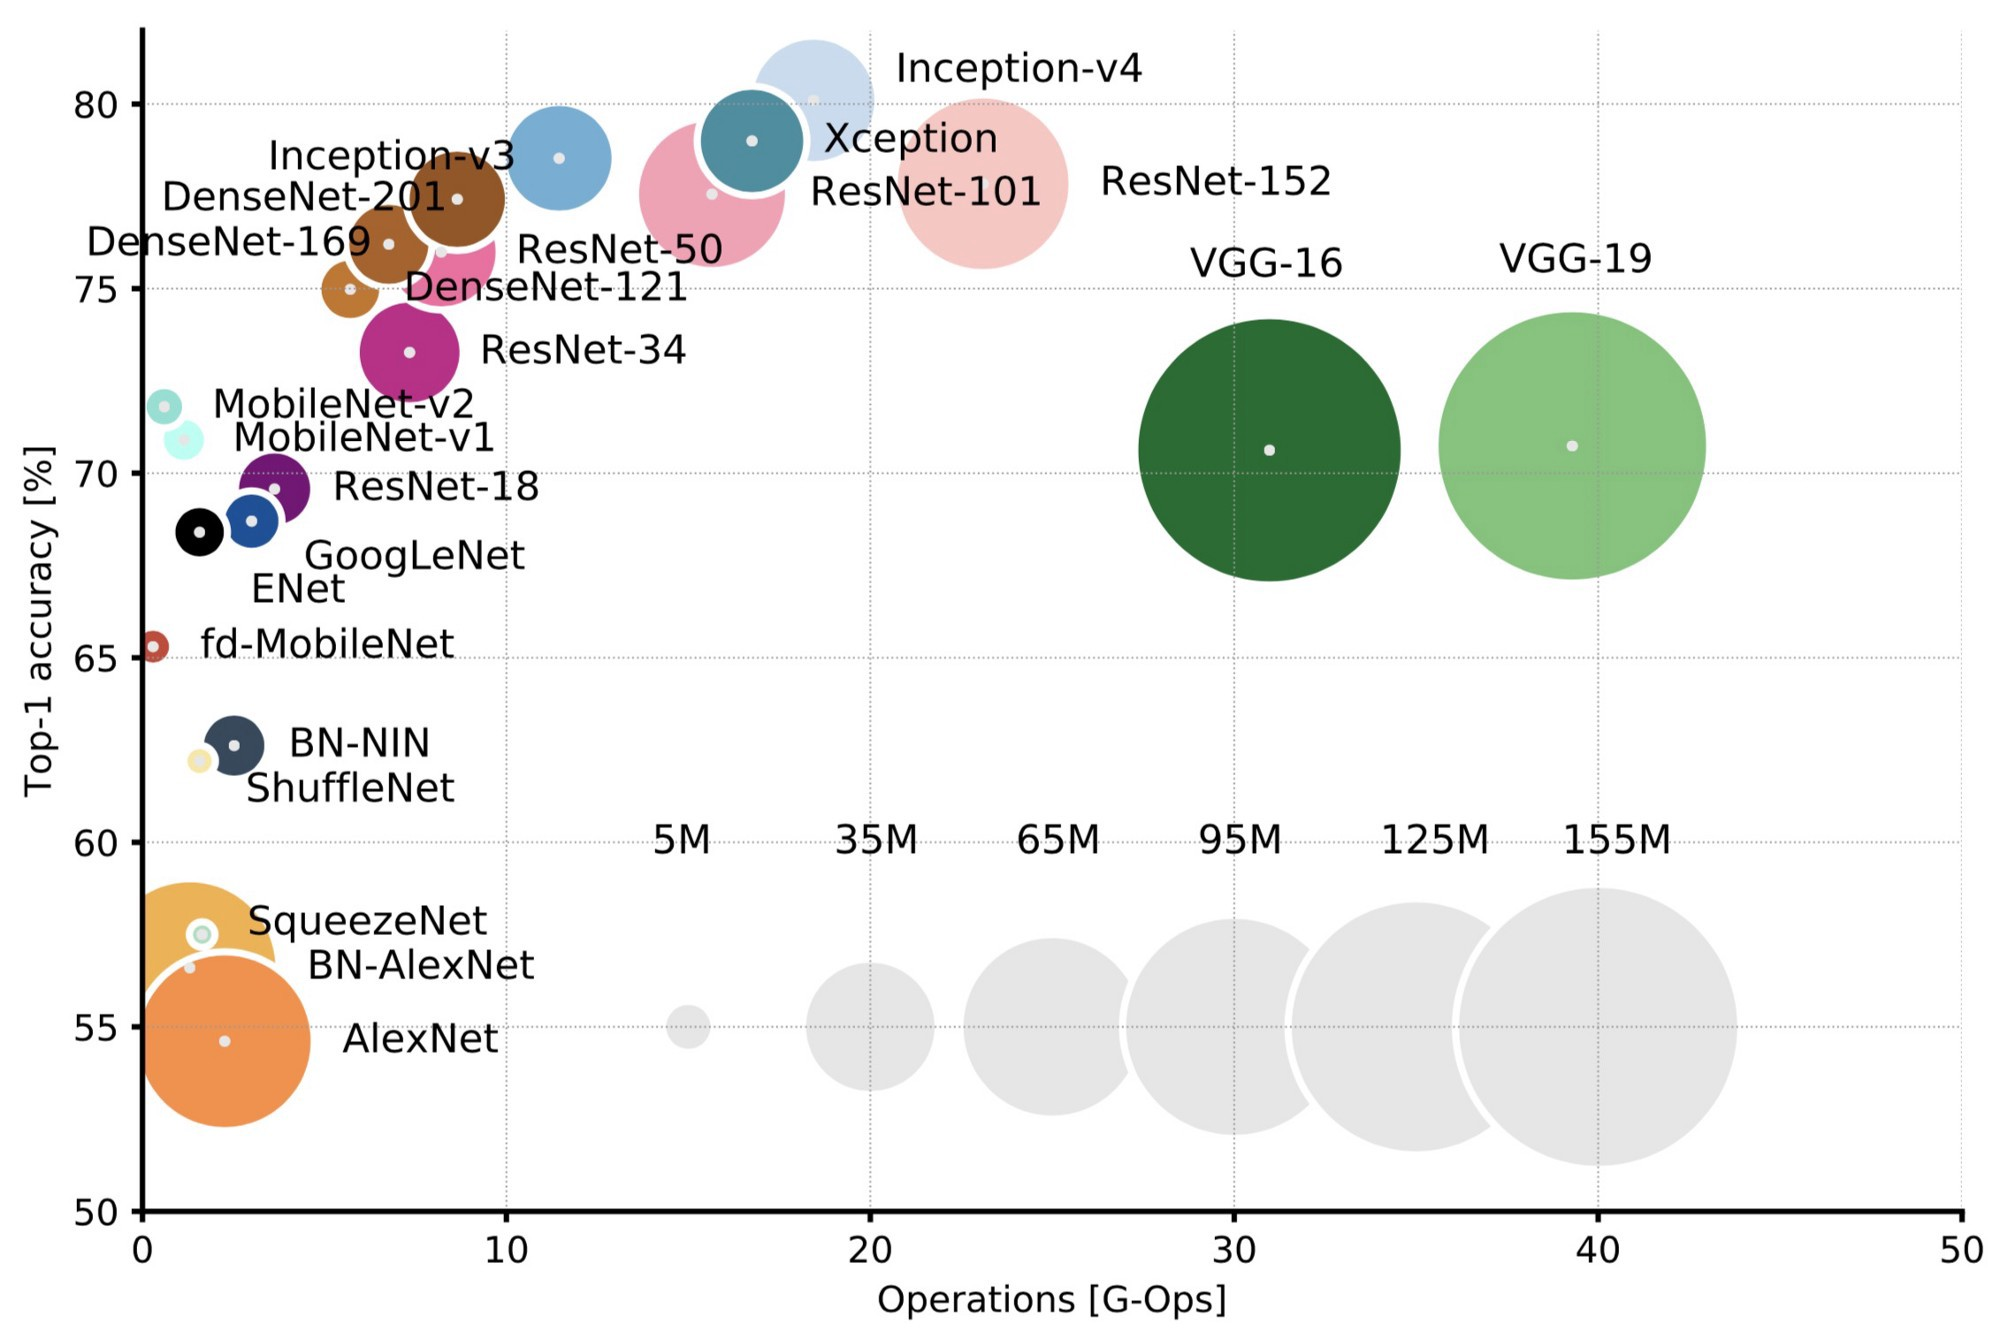
\includegraphics[width=1\columnwidth]{Famous_neural_networks} 
\caption[Les Réseaux Convolutifs sur ImageNet]{Les réseaux convolutifs d’un type particulier selon accuracy sur ImageNet).} 
\label{fig:Famous_neural_networks} 
\end{figure}

\paragraph{U-Net}
Il a été proposé par le département d’informatique de l’Université de Fribourg en Allemagne. C’est un réseau convolutif. C’est un réseau qui se compose d’une partie contractante et d’une voie expansive.
\begin{figure}[htb]
\centering 
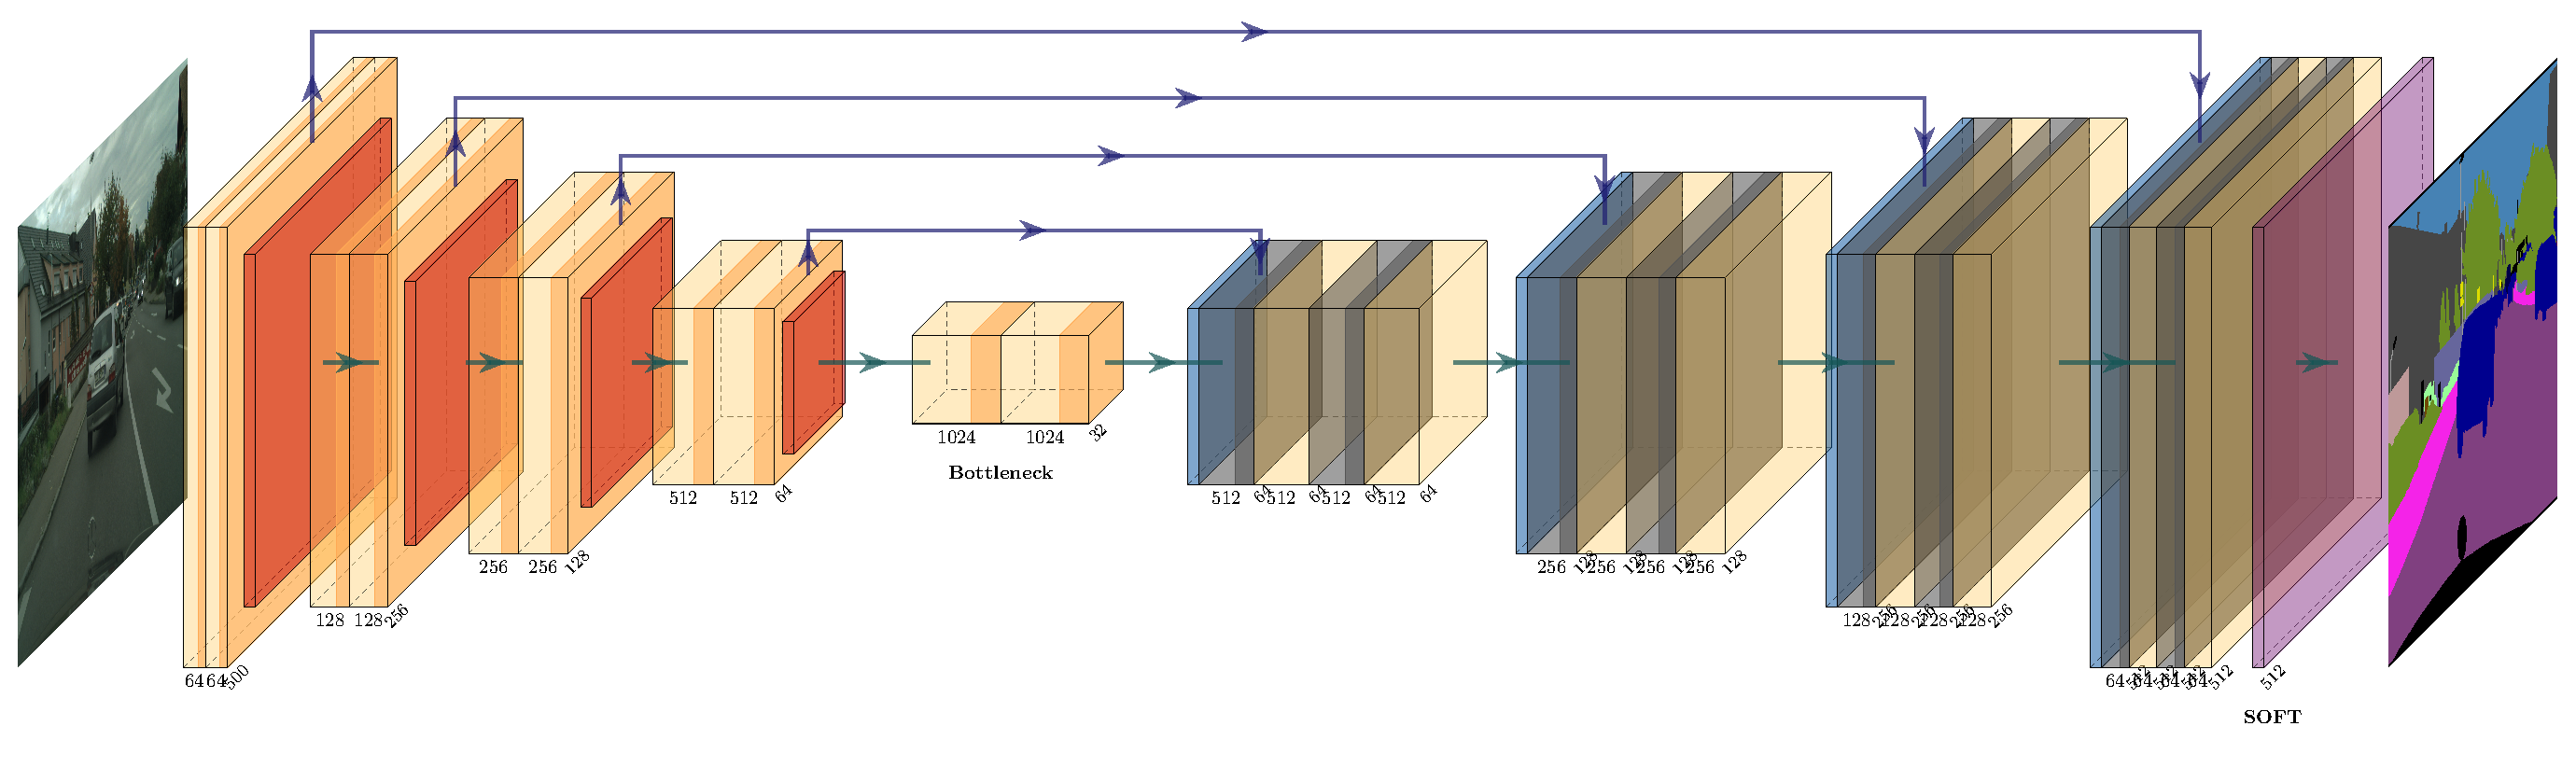
\includegraphics[width=1\columnwidth]{Unet_Xception} 
\caption[U-Net]{Un réseau U-Net pour Mask R-CNN. Le réseau encode puis décode l’image} 
\label{fig:Unet_Xception} 
\end{figure}
\paragraph{Xception}
Ce modèle représente une interprétation des modules Inception dans les réseaux neuronaux de convolution. Pour être simple, il marque une étape intermédiaire entre la convolution régulière et l’opération de convolution séparable en profondeur\cite{cho2017xception} (une convolution profonde suivie par une convolution par point).
\\
Inversement, une convolution séparable en profondeur peut être comprise comme un module d’Inception avec un grand nombre de tours maximum.
\\
Cette observation a mené à proposer une nouvelle architecture de réseau neuronal profond de convolution inspirée par Inception, où les modules d’Inception ont été remplacés avec les convolutions séparables profondes.
\\
Cette architecture, surnommé Xception, dépasse légèrement Inception V3 sur la base ImageNet (pour laquelle le réseau Inception V3 avait été fabriqué), et dépasse significativement Inception V3 sur des bases de données de classification d’image plus grande comprenant 350 millions d’images et 17000 classes.
\\
Comme l’architecture Xception a le même nombre de paramètres qu’Inception V3, les gains de performance sont essentiellement dus à l’augmentation des capacités plutôt qu’à un usage plus efficient des paramètres du modèle, d’où la réalisation du SOTA.

\paragraph{ResNet-50}
Il a été proposé par Kaiming He, un chercheur du laboratoire de Microsoft-Research à Beijing. C’est un standard de la reconnaissance d’image. Sa particularité est de comporter des connexions « saute-mouton » que l’on appelle connexions résiduelles\cite{LeCun_2019_qlma}, et qui court-circuitent des paires de couches.
 
\paragraph{DeepLabV3 plus}
Primo, il est composé d’une convolution Atrous\cite{deeplabv3plus2018} qui permet de contrôler explicitement la résolution à laquelle les réponses de features sont calculées à l’intérieur du \index{DCNN}\gls{DCNN} (Deep Convolutional Neural Networks). Ceci permet aussi d’élargir significativement le champ de vue des filtres à incorporer pour de plus large contexte sans augmentation du nombre de paramètres ou du nombre de calcul.
\begin{figure}[htb]
\centering 
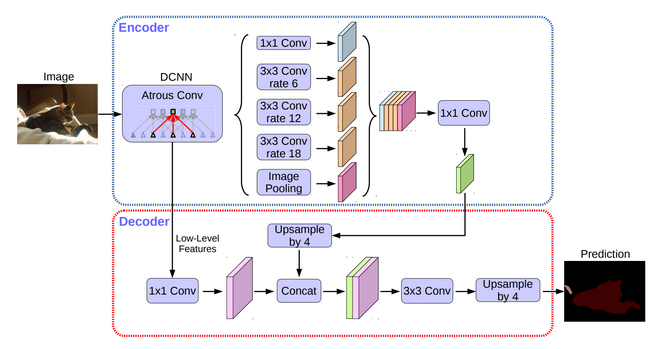
\includegraphics[width=1\columnwidth]{deeplabv3_plus} 
\caption[DeepLabV3 plus]{Le réseau neuronal \index{DeepLabV3}DeepLabV3 plus} 
\label{fig:deeplabv3_plus} 
\end{figure}
\paragraph{}Secundo, il propose ASPP pour \index{ASPP}\gls{ASPP}, qui segmente robustement des objets à de multiples échelles. ASPP pourvoit une couche convolutive de caractéristiques, en entrée, avec des filtres à des taux de multiple échantillonnage et des champs de vue efficaces, bien que capturant les objets aussi bien que le contexte de l’image à de multiples échelles.

\paragraph{}Tertio, la localisation des limites d’objets est améliorée en combinant des méthodes des DCNN et des modèles graphiques probabilistes. Le déploiement commun des combinaisons de max-pooling et de downsampling dans le DCNN aboutit à une invariance mais celle-ci impacte l’exactitude sur la localisation.
\\
Le réseau atténue ce problème en combinant les réponses à une couche finale DCNN avec un fully connected Conditional Random Field (CRF), laquelle donne des améliorations qualitatives et quantitatives dans la performance de localisation.

\paragraph{}Le système "\index{DeepLabV3}DeepLabV3 plus" règle le SOTA sur PASCAL VOC-2012 de la tâche de segmentation sémantique d’image. atteignant 79.7\% \index{mIoU}mIoU dans le jeu de test, et avance des résultats  sur 3 autres bases : PASCAL-Context, PASCAL-Person-Part, et Cityscapes.
\section{Les Encodeurs-Décodeurs}
\paragraph{}Nos réseaux utilisent l’architecture d’encodeur-décodeur\cite{zhang2020dive}. Le premier prend une entrée de taille variable et la conformise à un format, le second mappe l’état encodé (dans un état contraint) vers une séquence de longueur variable.

\begin{figure}[htb]
\centering 
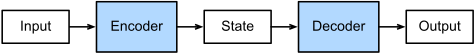
\includegraphics[width=1\columnwidth]{encoder-decoder} 
\caption[L’architecture encoder-decoder]{L’architecture encoder-decoder} 
\label{fig:data_augmentation} 
\end{figure}
\paragraph{}Dans la bibliothèque \index{Keras}Keras, son intégration se fait comme suit :

\inputminted[
frame=lines,
framesep=2mm,
baselinestretch=1,
fontsize=\footnotesize,
linenos=true,
firstnumber=last
]{python}{code/enc_dec.py}

\section{Nos Masques R-CNN}
\paragraph{}Pour réaliser notre travail de segmentation d’image, nous avons réduit le nombre de classes de nos masques à 8, et ceci de façon astucieuse : Plutôt que de "mapper" chaque pixel des masques à 32 dimensions, nous avons utilisé les fichiers de cotation de nos polygones, ces premiers, qui sont au format JSON, nous leur avons "mapper" les catégories dans un tableau de valeur, sérialisé lui-aussi en JSON. Finalement, ce tableau est d’une dimension plus raisonnable que le nombre de pixel d’une image, qui dans Citiscapes, est de $1024x2048$ pixels.
\\
Il ne nous restait ensuite plus qu’à utiliser la fonction fillPoly d’openCV pour créer nos nouveaux masques, ceux-ci portant seulement les 8 dimensions nécessaires à notre travail de segmentation d’image. Cette technique nous a permis d’économiser beaucoup de temps de calcul. Nous avons élaboré cette dernière en recherchant comment optimiser le nombre de lecture/écriture sur le disque dur pour limiter le nombre d’accès disque.

\inputminted[
frame=lines,
framesep=2mm,
baselinestretch=1,
fontsize=\footnotesize,
linenos=true,
firstnumber=last
]{python}{code/mask_preparation.py}

\paragraph{}Grâce à ces préparatifs, nous avons obtenu un jeu de données d’entraînement et de validation. Pour pallier aux $500$ masques de tests complètement opaques de la base fournie, nous avons tiré aléatoirement $500$ images à chaque entraînement parmi les données d’entraînement. Les images furent isolées ipso facto, car une utilisation post-apprentissage est requise en vue de réaliser les mesures sur données de test, donc des performances (\index{mIoU}mIoU et \index{S{\o}rensen-Dice}S{\o}rensen-Dice de modèle de \index{Deep Learning}\gls{DL}.

\section{Data Augmentation}
\paragraph{}Pour réaliser l’augmentation de données nous avons réalisé des retouches d’images en série pour toutes les images de l’entraînement, soit $2475$ images. Nous avons testé plusieurs bibliothèques avant de retenir \href{https://imgaug.readthedocs.io/en/latest/}{imgaug}. Nous avons été limité dans notre choix par la différence de dimension entre les images d’entrée et de sortie, elle ne respecte pas la structure (la signature) de la méthode centrale de la classe ImageDataGenerator de la bibliothèque \index{TensorFlow}TensorFlow. Cependant, l’égalisation des dimensions d’entrée et de sortie semble être une piste pour travailler la data augmentation en temps réel, même si cela nous rapprocherait de la méthode dont on use pour un réseau \index{GAN}GAN. Par contre, dans notre situation, nous avons chargé le double du nombre de fichier originaux sur le disque-dur, du moins dans les apprentissages qui ont eu lieu en mode "augmentation de données".

\inputminted[
frame=lines,
framesep=2mm,
baselinestretch=1,
fontsize=\footnotesize,
linenos=true,
firstnumber=last
]{python}{code/data_augmentation.py}


\begin{figure}[htb]
\centering 
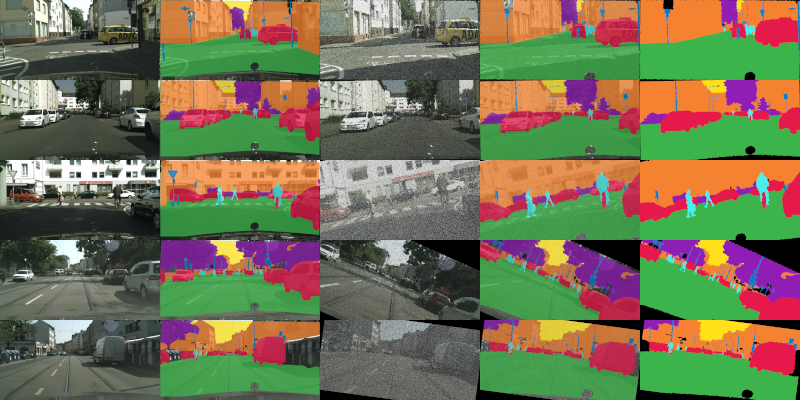
\includegraphics[width=1\columnwidth]{data_augmentation} 
\caption[Data Augmentation]{Data Augmentation des Images et des Masks R-CNN}
\label{fig:data_augmentation} 
\end{figure}
\section{Data Generator}
Pour permettre le chargement de nos données en cachant la complexité du code, nous avons créé plusieurs classes et un fichier regroupant les fonctions statiques. Ainsi notre classe DataGenerator nous permet-elle d’utiliser une écriture claire avec un switch dans une fonction appelante \_\_call\_\_ et des méthodes utilisant le pattern d’objet Factory pour masquer la complexité du code dans notre classe, laquelle ne contient que le concept auquel nous faisons référence lors du chargement de nos data, dont le code de l’action plus bas niveau se trouve dans un fichier regroupant les fonctions statiques (tools).  Dans notre code, c’est le cadriciel DVC qui joue le rôle de commande à travers un pattern "Command" cette fois, mais l’idée reste la même bien que le concept soit de plus haut niveau.\\
Les deux patterns sont exposés dans le schéma UML suivant :

\begin{figure}[htb]
\centering 
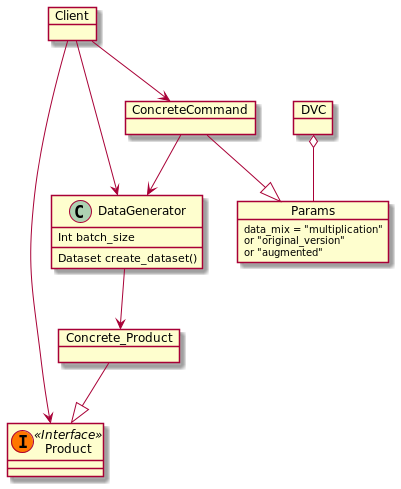
\includegraphics[width=0.7\columnwidth]{factory} 
\caption[Factory Pattern et Data Generator]{Utilisation de pattern Factory et Command pour le DataGenerator} 
\label{fig:data_augmentation} 
\end{figure}

Ci-dessous un extrait de la classe DataGenerator.
\inputminted[
frame=lines,
framesep=2mm,
baselinestretch=1,
fontsize=\footnotesize,
linenos=true,
firstnumber=last
]{python}{code/data_generator.py}

Ce genre d’écriture est utilisé en Programmation Orientée Objet et représente un ensemble de bonnes pratiques de codage pour la maintenabilité et notamment le travail en équipe.
\section{Comparaison}
\paragraph{}Nous avons travaillé deux sortes d’algorithmes. Le premier, simple et classique, est un réseau \index{R-CNN}R-CNN, sur le modèle de \index{U-Net}U-Net et \index{Xception}Xception. Il utilise la structure du modèle, mais sans le modèle pré-entraîné. Le second est plus complexe car il comporte une méthode d’apprentissage par \index{Transfer Learning}transfer learning, celui-ci est obtenu par le modèle pré-entraîné \index{ResNet 50}ResNet 50, sur une structure globale de \index{DeepLabV3} plus.
\paragraph{}Nous avons effectué beaucoup d’expériences pour régler nos hypers paramètres d’apprentissage profond\ref{experiments}. Nous avons de plus rangé les expériences selon le type de data en présence, car nous voulions mettre en évidence les améliorations apportées par l’augmentation de data.

\begin{table}[h]\center
\begin{tabular}{@{}lllllll@{}}
\toprule
name    & mIoU & dice & time    & data\_mix         & optim\_type & learning\_rate \\ \midrule
deeplab & 0,6  & 0,7  & 1586,42 & original\_version & rmsprop     & 0,00019        \\
deeplab & 0,62 & 0,71 & 1589,59 & multiplication    & rmsprop     & 0,00019        \\
deeplab & 0,61 & 0,7  & 1686,6  & original\_version & nadam       & 8E-05          \\
deeplab & 0,6  & 0,7  & 1698,6  & multiplication    & nadam       & 8E-05          \\
UNet    & 0,54 & 0,63 & 995,57  & original\_version & adam        & 0,00015        \\
UNet    & 0,48 & 0,58 & 996,59  & multiplication    & adam        & 0,00015        \\
UNet    & 0,54 & 0,63 & 997,76  & original\_version & rmsprop     & 0,00037        \\
UNet    & 0,5  & 0,6  & 991,54  & multiplication    & rmsprop     & 0,00037        \\ \bottomrule
\end{tabular}
\caption[Comparaison de quelques optimisations]{Comparaison de quelques optimisations : Notre meilleure performance est avec augmentation de data et optimiseur rmsprop}
\label{comparaison_table}
\end{table}

\paragraph{}Le tableau \ref{comparaison} nous montre que le meilleur score parmi nos modèles est de $71$\% pour le \index{S{\o}rensen-Dice} coefficient de Dice et de $62$\% pour le \index{mIoU}mIoU. Nous pouvons nous apercevoir que l’augmentation de data a une réelle valeur ajoutée seulement pour les cas où le taux d’apprentissage est bas ($>2e^{-4}$) et en utilisant l’optimiseur rmsprop, dont la particularité est de supporter la mise à jour, même pour une valeur nulle du gradient, quand l’optimiseur est dans une implémentation dense.

\begin{figure}[htb]
\centering
\subfloat[Coût]{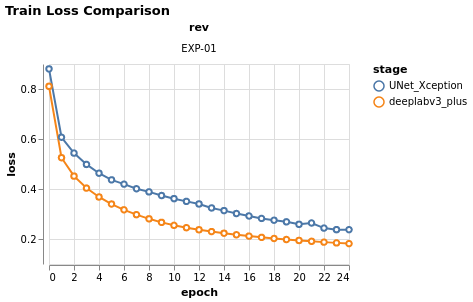
\includegraphics[width=.45\columnwidth]{loss}} \quad
\subfloat[Exactitude]{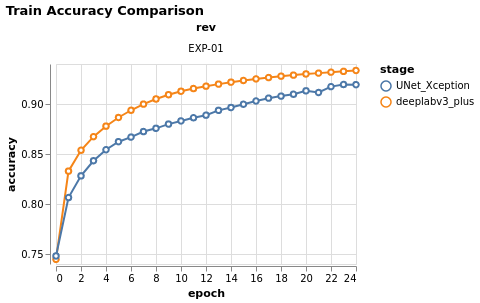
\includegraphics[width=.45\columnwidth]{accuracy}} \\
\subfloat[Balanced]{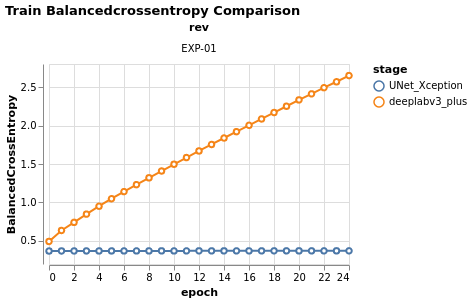
\includegraphics[width=.45\columnwidth]{balanced}} \quad
\subfloat[Weighted]{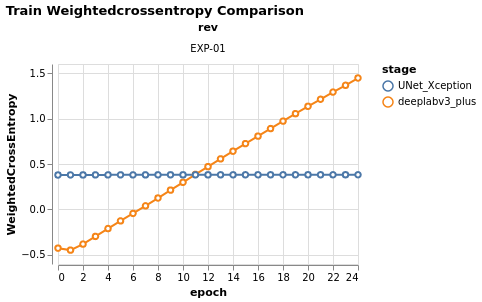
\includegraphics[width=.45\columnwidth]{weighted}}
\caption[Mesure des Performances]{Comparaison de métriques et de coûts des meilleurs modèles pour chaque réseau.} 
\label{fig:comparaison}
\end{figure}

\section{Conclusion}
\paragraph{}Dans cet article, nous avons présenté nos différentes approches, celle de U-Net avec Xception et celle de DeepLab avec ResNet. De plus nous avons parcouru l’histoire des réseaux convolutifs du siècle dernier à nos jours. Nous avons pris le soin d’énumérer les réseaux ayant dépassés les SOTA puis de nous concentrer sur une sélection parmi une poignée d’entre-eux\ref{comparaison}.

\paragraph{}Ensuite nous avons mis l’accent sur la construction d’une base de données augmentées\ref{data_augmentation} et sur l’amélioration notable qu’elle pourvoie à l’apprentissage du modèle\ref{comparaison_table}.

\paragraph{}Pour poursuivre cette étude, il serait utile de modifier l’usage du ResNet-50 par son petit-frère le ResNet-152, comportant plus de couches de convolution. De plus, il nous semblerait utile de tester les performances d’autres réseaux pré-entraînés dans le modèle utilisé, ou encore de poursuivre l’entraînement en réduisant encore un peu plus le taux d’apprentissage.

\paragraph{}De plus, il nous paraît pertinent d’imaginer l’ajout d’une autre série de transformation au-moins, à nos données, pour leurs formuler de plus nombreuses augmentations, puisqu’en l’occurrence, le réseau semble être plus performant quand il a plus de data.
\paragraph{}Enfin, pour nous intégrer au mode de lecture en temps réel de notre voiture autonome, nous envisageons de réduire drastiquement la dimension dans les 3 axes du tenseur représentant les images d’entrée, pour assurer une rapidité d’exécution, au moment du fonctionnement du véhicule électrique.
\section{Annexe}

\begin{landscape}
\begin{table}
\begin{tabular}{|l|l|l|l|l|l|l|r|l|l|r|l|l|l|l|}\toprule{} & Experiment &     BCE &     WCE & accuracy &   loss &  mIoU &  step &     time &  dice &  epochs &          data\_mix &      name & optim\_type & learning\_rate \\\midrule 0  &  exp-7bc0f &  10,604 &   8,728 &    0,934 &  0,173 &   0,6 &    19 &  1724,62 &  0,69 &      20 &  original\_version &     deeplab &      nadam &       0,00085 \\1  &  exp-3ca96 &  10,708 &   8,916 &    0,934 &  0,176 &  0,59 &    19 &   1697,2 &  0,69 &      20 &    multiplication &     deeplab &      nadam &       0,00085 \\2  &  exp-d0e65 &   5,960 &   4,429 &    0,940 &  0,153 &  0,61 &    19 &  1533,93 &   0,7 &      20 &  original\_version &     deeplab &       adam &       0,00015 \\3  &  exp-c9ac1 &   6,044 &   4,608 &    0,940 &  0,155 &  0,61 &    19 &  1522,94 &   0,7 &      20 &    multiplication &     deeplab &       adam &       0,00015 \\4  &  exp-e321a &   4,251 &   2,994 &    0,943 &  0,142 &  0,61 &    19 &   1686,6 &   0,7 &      20 &  original\_version &     deeplab &      nadam &         8E-05 \\5  &  exp-c76d4 &   3,956 &   2,605 &    0,943 &  0,142 &   0,6 &    19 &   1698,6 &   0,7 &      20 &    multiplication &     deeplab &      nadam &         8E-05 \\6  &  exp-c6a43 &  21,457 &  20,301 &    0,940 &  0,151 &  0,61 &    19 &  1585,62 &   0,7 &      20 &  original\_version &     deeplab &    rmsprop &       0,00037 \\7  &  exp-e4dff &  20,901 &  19,685 &    0,941 &  0,150 &   0,6 &    19 &  1586,27 &   0,7 &      20 &    multiplication &     deeplab &    rmsprop &       0,00037 \\8  &  exp-e93a2 &   1,452 &   0,536 &    0,822 &  0,550 &  0,45 &    19 &  1486,55 &  0,55 &      20 &  original\_version &     deeplab &        sgd &       0,00047 \\9  &  exp-78dfd &   1,412 &   0,528 &    0,823 &  0,546 &  0,45 &    19 &  1491,36 &  0,55 &      20 &    multiplication &     deeplab &        sgd &       0,00047 \\10 &  exp-70cad &   1,318 &   0,171 &    0,822 &  0,558 &  0,46 &    19 &   1535,1 &  0,55 &      20 &  original\_version &     deeplab &   adadelta &       0,00082 \\11 &  exp-92faf &   1,081 &  -0,241 &    0,821 &  0,561 &  0,46 &    19 &  1537,94 &  0,55 &      20 &    multiplication &     deeplab &   adadelta &       0,00082 \\12 &  exp-a0f8c &  17,876 &  16,164 &    0,943 &  0,141 &   0,6 &    19 &  1586,42 &   0,7 &      20 &  original\_version &     deeplab &    rmsprop &       0,00019 \\13 &  exp-34ef2 &  17,287 &  15,537 &    0,943 &  0,142 &  0,62 &    19 &  1589,59 &  0,71 &      20 &    multiplication &     deeplab &    rmsprop &       0,00019 \\14 &  exp-db829 &   1,542 &   0,205 &    0,825 &  0,539 &  0,46 &    19 &  1504,13 &  0,55 &      20 &  original\_version &     deeplab &        sgd &        0,0005 \\15 &  exp-29f17 &   1,666 &   0,364 &    0,824 &  0,541 &  0,46 &    19 &   1494,5 &  0,56 &      20 &    multiplication &     deeplab &        sgd &        0,0005 \\16 &  exp-ba3d8 &   1,165 &   0,381 &    0,911 &  0,264 &  0,54 &    19 &    991,8 &  0,63 &      20 &  original\_version &  U-Net &      nadam &       0,00085 \\17 &  exp-53c97 &   1,164 &   0,382 &    0,911 &  0,267 &  0,51 &    19 &  1008,77 &  0,61 &      20 &    multiplication &  U-Net &      nadam &       0,00085 \\18 &  exp-d8c86 &   0,624 &   0,382 &    0,912 &  0,261 &  0,54 &    19 &   995,57 &  0,63 &      20 &  original\_version &  U-Net &       adam &       0,00015 \\19 &  exp-7c564 &   0,624 &   0,381 &    0,910 &  0,268 &  0,48 &    19 &   996,59 &  0,58 &      20 &    multiplication &  U-Net &       adam &       0,00015 \\20 &  exp-b4ea4 &   0,299 &   0,382 &    0,912 &  0,263 &  0,53 &    19 &   990,16 &  0,62 &      20 &  original\_version &  U-Net &      nadam &         8E-05 \\21 &  exp-8d64e &   0,299 &   0,381 &    0,913 &  0,259 &  0,46 &    19 &   992,64 &  0,56 &      20 &    multiplication &  U-Net &      nadam &         8E-05 \\22 &  exp-30f96 &   1,382 &   0,381 &    0,910 &  0,268 &  0,54 &    19 &   997,76 &  0,63 &      20 &  original\_version &  U-Net &    rmsprop &       0,00037 \\23 &  exp-f13b2 &   1,381 &   0,381 &    0,910 &  0,267 &   0,5 &    19 &   991,54 &   0,6 &      20 &    multiplication &  U-Net &    rmsprop &       0,00037 \\24 &  exp-0ef32 &   0,515 &   0,382 &    0,913 &  0,260 &  0,49 &    19 &   992,04 &  0,59 &      20 &  original\_version &  U-Net &        sgd &       0,00047 \\25 &  exp-42da6 &   0,516 &   0,381 &    0,917 &  0,245 &   0,5 &    19 &   992,42 &   0,6 &      20 &    multiplication &  U-Net &        sgd &       0,00047 \\26 &  exp-90d63 &   0,696 &   0,381 &    0,913 &  0,261 &  0,52 &    19 &   990,81 &  0,62 &      20 &  original\_version &  U-Net &   adadelta &       0,00082 \\27 &  exp-b8f91 &   0,696 &   0,381 &    0,913 &  0,259 &   0,5 &    19 &   994,91 &   0,6 &      20 &    multiplication &  U-Net &   adadelta &       0,00082 \\28 &  exp-77c21 &   1,600 &   0,381 &    0,911 &  0,265 &  0,52 &    19 &   990,24 &  0,61 &      20 &  original\_version &  U-Net &    rmsprop &       0,00019 \\29 &  exp-7043e &   1,600 &   0,381 &    0,913 &  0,257 &  0,49 &    19 &    989,4 &  0,59 &      20 &    multiplication &  U-Net &    rmsprop &       0,00019 \\30 &  exp-78211 &   0,840 &   0,381 &    0,910 &  0,268 &  0,51 &    19 &   992,08 &  0,61 &      20 &  original\_version &  U-Net &        sgd &        0,0005 \\31 &  exp-5ca61 &   0,841 &   0,381 &    0,913 &  0,260 &  0,49 &    19 &   996,07 &  0,59 &      20 &    multiplication &  U-Net &        sgd &        0,0005 \\\bottomrule\end{tabular}\caption{Tableau d’expérimentations}\label{experiments}\end{table}
\end{landscape}

\printindex
\clearpage
\printglossaries

\renewcommand{\refname}{\spacedlowsmallcaps{References}} 

\bibliographystyle{unsrt}

\bibliography{sample.bib}


\end{document}